% OCR-assisted facsimile of the Intellivision Keyboard Component Service Manual.
% Build from keyboard/: latexmk -pdf KeyboardComponentServiceManual-OCR.tex
\documentclass[letterpaper,11pt]{article}

\usepackage[T1]{fontenc}
\usepackage{geometry}
\usepackage{hyperref}
\usepackage{pdfpages}
\geometry{margin=1in}
\hypersetup{colorlinks=true,linkcolor=black,urlcolor=blue,pdftitle={Intellivision Keyboard Component Service Manual -- OCR-assisted LaTeX Facsimile}}

\begin{document}

\begin{titlepage}
  \centering
  \vspace*{0.18\textheight}
  {\LARGE\bfseries Intellivision Keyboard Component\par}
  \vspace{0.4em}
  {\Large Service Manual\par}
  \vspace{1.5em}
  {\large OCR-assisted LaTeX facsimile edition\par}
  \vfill
  \begin{minipage}{0.82\textwidth}
    \small
    Every original manual page and figure is retained as a page image. The
    embedded source additionally carries a machine-generated OCR text layer,
    making the resulting PDF searchable and selectable.

    \medskip
    OCR source: \texttt{KeyboardComponentServiceManual-OCR-source.pdf}\\
    Plain-text sidecar: \texttt{KeyboardComponentServiceManual-OCR.txt}

    \medskip
    \textbf{Verification requirement:} OCR is an aid to discovery, not a
    replacement for visual inspection. Consult the page image for component
    names, part numbers, circuit values, diagrams, and tables.
  \end{minipage}
  \vfill
  {\small Repository edition, \today\par}
\end{titlepage}

\pdfbookmark[0]{OCR-assisted service manual facsimile}{manual}
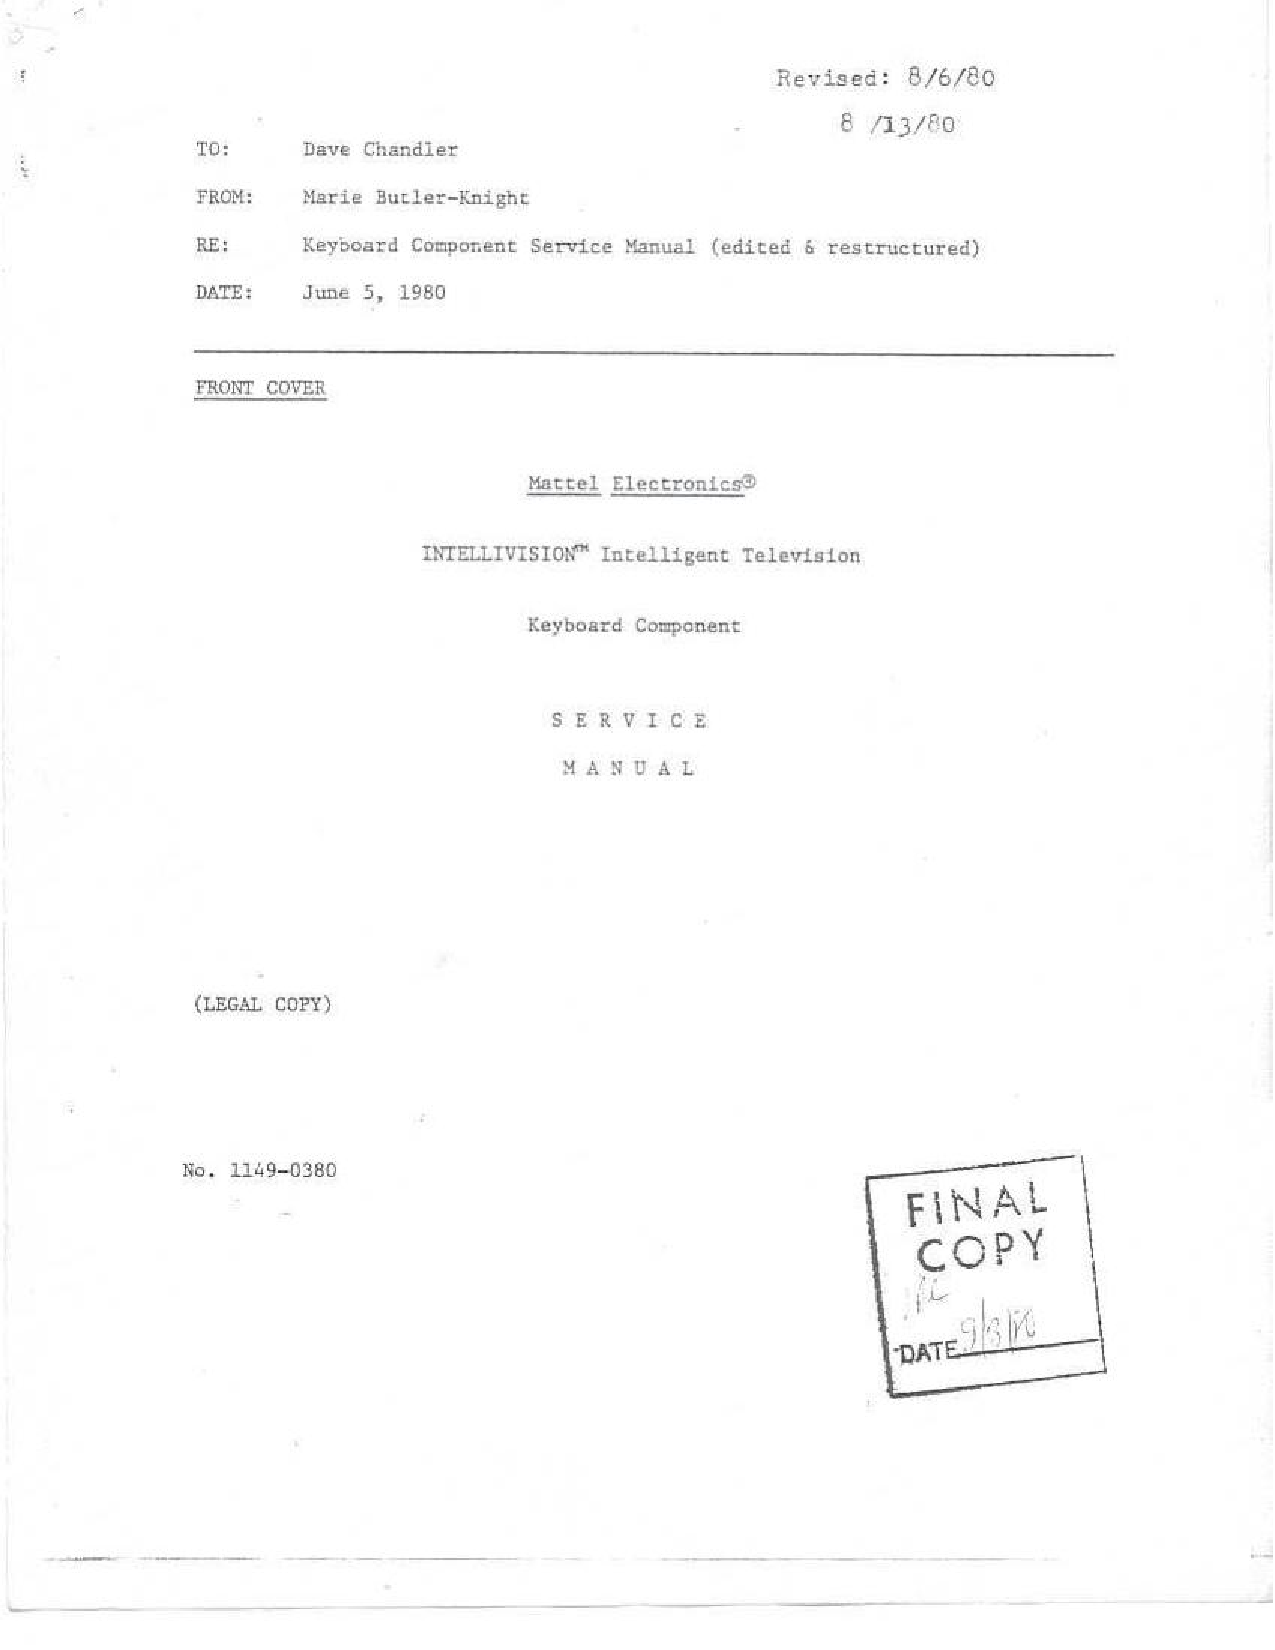
\includepdf[pages=-,pagecommand={},fitpaper=true]{KeyboardComponentServiceManual-OCR-source.pdf}

\end{document}
